\chapter{Implementacija i korisničko sučelje}
		
		
		\section{Korištene tehnologije i alati}
			{
				Komunikacija u timu je ostvarena korištenjem aplikacija Discord\footnote{\url{https://discord.com/}} i GoogleMeet\footnote{\url{https://meet.google.com/}}.
				Komunikacija s asistentom grupe je ostvarena korištenjem aplikacije MicrosoftOutlook\footnote{\url{https://outlook.live.com/owa/}}.
				Za izradu sekvencijskih UML dijagrama i UML dijagrama obrazaca uporabe korišten je alat Astah UML\footnote{\url{https://astah.net/products/astah-uml/}}. Za izradu UML dijagrama razreda korišten je alat IntelliJ\footnote{\url{https://www.jetbrains.com/idea/}}. Za izradu dijagrama razmještaja korišten je alat VisualParadigmOnline\footnote{\url{https://online.visual-paradigm.com/}}, a za izradu dijagrama aktivnosti korišten je program Pages razvijen od strane Apple Inc.\footnote{\url{https://www.apple.com/pages/}}.
				Za izradu modela baze podataka korišten je alat ERDPlus\footnote{\url{https://erdplus.com/}}.
				Za upravljanje izvornim kodom korišten je alat Git\footnote{\url{https://git-scm.com/}}. Udaljeni repozitorij projekta nalazi se na platformi Gitlab\footnote{\url{https://gitlab.com/}} koja je korištena i za upravljanje zadacima na projektu.
				Kao razvojno okruženje na backendu je korišten IntelliJ, a na frontendu je korišten Visual Studio Code\footnote{\url{https://code.visualstudio.com/}}. Tehnologije korištene za razvoj backenda su radni okvir Spring Boot\footnote{\url{https://spring.io/projects/spring-boot}} i programski jezik Java\footnote{\url{https://www.java.com/en/}}. Tehologije korištene za razvoj frontenda su biblioteka React\footnote{\url{https://reactjs.org/}} i programski jezik JavaScript\footnote{\url{https://www.javascript.com/}}.
				\eject
				Za automatizirano testiranje cjelokupne aplikacije korišten je alat Selenium IDE\footnote{\url{https://www.selenium.dev/selenium-ide/}} te programski jezik Java. 
				Za automatizirano testiranje komponenti korišten je alat JUnit\footnote{\url{https://junit.org/junit5/}} te programski jezik Java.
				Za ručno testiranje korišten je alat ReqBin\footnote{\url{https://reqbin.com/}} te programski jezik Java.
				Za puštanje aplikacije u pogon korištena je platforma MicrosoftAzure\footnote{\url{https://azure.microsoft.com/en-us}}.
		    }
			
			\eject 
		
	
		\section{Ispitivanje programskog rješenja}
			
			\subsection{Ispitivanje komponenti}
			\normalfont{Ispitivanje komponenti ostvareno je pomoću Spring Boot i JUnit 5 alata za ispitivanje. \newline Na slikama \ref{fig:TestCompatibleStationLinkSatellite1} i \ref{fig:TestCompatibleStationLinkSatellite2} prikazani su isječci koda iz testa koji provjerava ispravnost spajanja i dohvaćanja kompatibilne trojke (satelit, link i stanica). Slika \ref{fig:TestCompatibleStationLinkSatellite1} prikazuje dva slučaja: 1. kada satelit, onosno njegovi transmiteri, nisu kompatibilni s linkovima koji se nalaze u bazi. Očekivani rezultat ovog slučaja je prazan set kompatibilnih likova. Te 2. kada postoji link koji je kompatibilan s transmiterom uz očekivani rezultat da set kompatibilnih likova sarži točno jedan link koji je jednak linku kojeg stvaramo u ovom testu. Slika \ref{fig:TestCompatibleStationLinkSatellite2} također prikazuje dva slučaja: 1. kada za određeni link ne postoje kompatibilne stanice, odnosno niti jedna antena neke stanice nije kompatibilna sa zadanim linkom. Očekivani rezultat u ovom slučaju je prazan set kompatibilnih stanica. Te 2. kada postoji stanica s kojom je zadani link kompatibilan. Očekivani rezultat ovog testa je da će set kompatibilnih stanica za zadani link sadržavati jednu stanicu koja je jednaka stanici koju na početnu testa stvaramo.}

            \begin{figure}[H]
					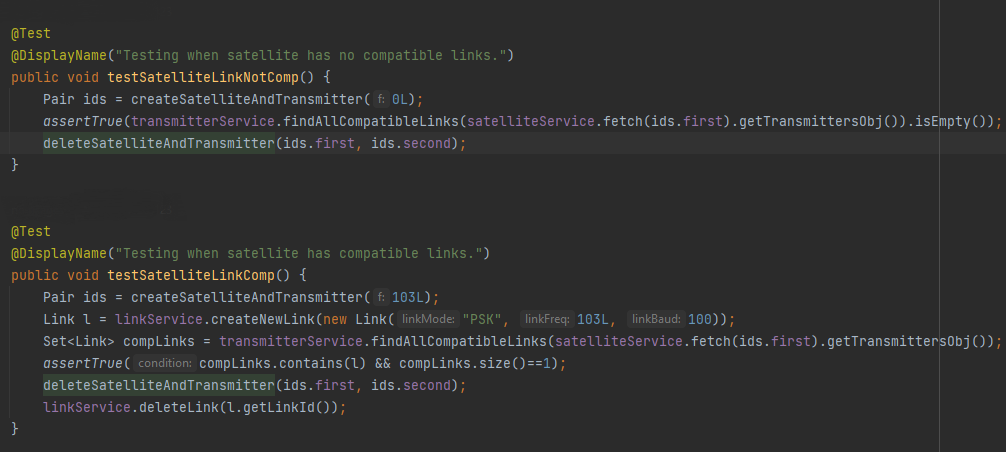
\includegraphics[width=\linewidth]{TestCompatibleStationLinkSatellite1.png}
					\caption{Testiranje spajanja i dohvaćanja kompatibilnih satelita i linkova}
					\label{fig:TestCompatibleStationLinkSatellite1}
				\end{figure}
            \begin{figure}[H]
					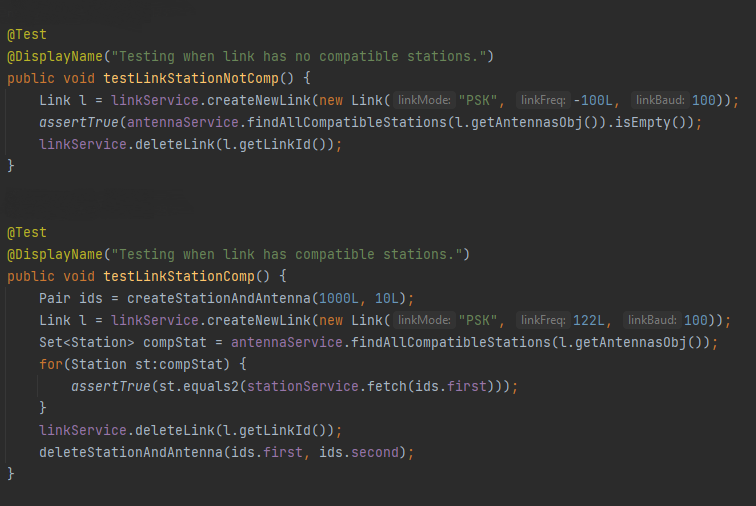
\includegraphics[width=\linewidth]{TestCompatibleStationLinkSatellite2.png}
					\caption{Testiranje spajanja i dohvaćanja kompatibilnih stanica i linkova}
					\label{fig:TestCompatibleStationLinkSatellite2}
				\end{figure}
			
			\normalfont{Na slici \ref{fig:TestStationChecker} prikazano je testiranje funkcionalnosti ispitivanja jednakosti stanica koje su spremljene u bazi u odnosu na stanice koje dohvaćamo sa SatNOGS API-ja. Za prvi test pretpostavka je da stanica s id-jem 6 postoji i u bazi satcom aplikacije i u bazi SatNOGS-a pa je sukladno tome očekivani rezultat istina, tj. stanice su jednake. Pretpostavka za drugi test je da smo u satnogs bazi promijenili barem jedan podatak stanice s id-jem 9 pa je zbog toga očekivai rezultat laž, odnosno da stanice nisu jednake. Pretpostavka za treći test je da smo u satnogs bazi promijenili barem jedan podatak neke antene koja pripada stanici s id-jem 12, tako da možemo očekivati da će rezultat ponovno biti laž, tj. stanice nisu jednake.}

            \begin{figure}[H]
					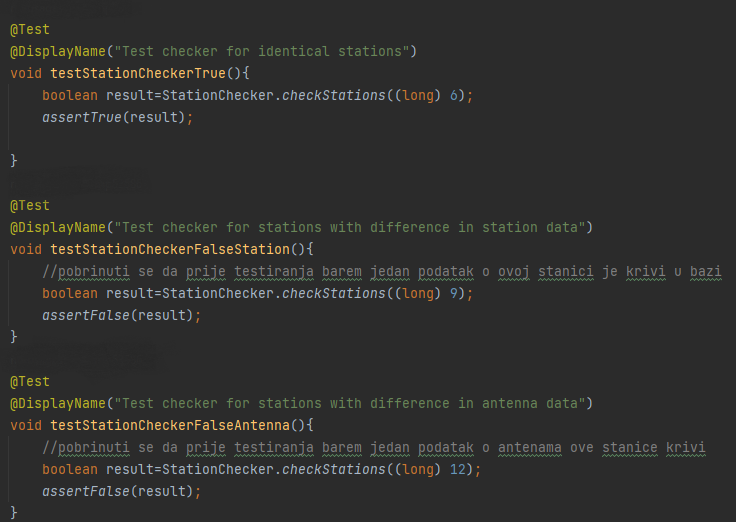
\includegraphics[width=\linewidth]{TestStationChecker.png}
					\caption{Testiranje ispitivanja jednakosti stanica u bazi i na SatNOGS API-ju}
					\label{fig:TestStationChecker}
				\end{figure}
				
			\normalfont{Na slici \ref{fig:TestMessageSaveToDB} prikazano je testiranje spremanja poruke u bazu. Prvi test pokriva slučaj spremanja kada su svi atributi modela Message ispravno postavljeni i očekivani rezultat nakon spremanja je da se u bazi nalazi poruka koja je jednaka onoj koju smo željeli spremiti. Drugi test prikazuje da se u slučaju pokušaja spremanja poruke koja nema sve atribute zadane, konkretno u ovom testnom primjeru atribut satelliteName je null, baca iznimka IllegalArgumentException.}

            \begin{figure}[H]
					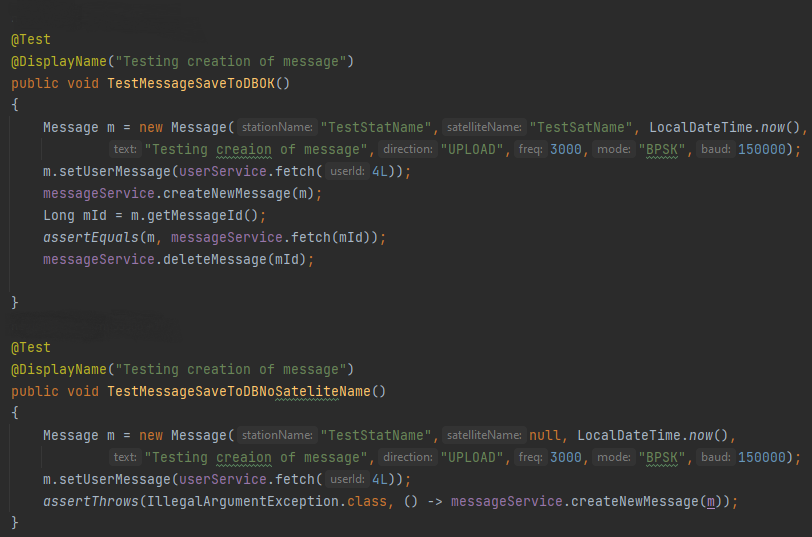
\includegraphics[width=\linewidth]{TestMessageSaveToDB.png}
					\caption{Testiranje spremanja poruka u bazu. }
					\label{fig:TestMessageSaveToDB}
				\end{figure}
				
			\normalfont{Na slikama \ref{fig:TestCommunicationWithSatellite1} i \ref{fig:TestCommunicationWithSatellite2} prikazano je testiranje komunikacije sa serverom kojem šaljemo poruke, tj. koji "glumi" satelit. Test na slici \ref{fig:TestCommunicationWithSatellite1} prikazuje da ako nedostaje neki od argumenata u poruci koju šaljemo, server će vratiti null kao odgovor. Test na slici \ref{fig:TestCommunicationWithSatellite2} prikazuje da ako pošaljemo ispravnu poruku, server će vratiti odgovor koji nije null.}

            \begin{figure}[H]
					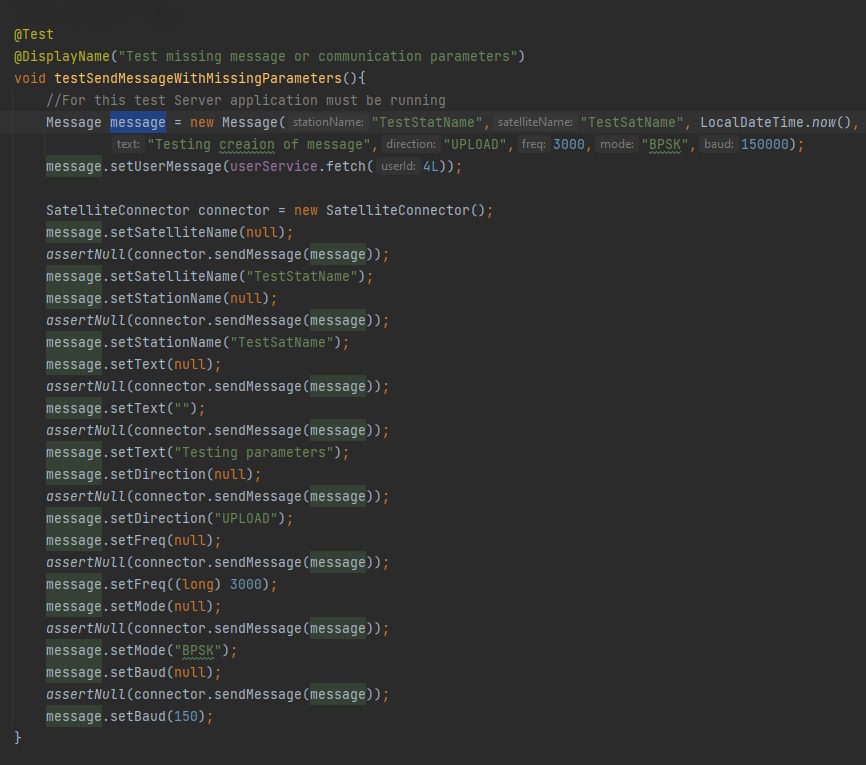
\includegraphics[width=\linewidth]{TestCommunicationWithSatellite1.png}
					\caption{Testiranje neispravne komunikacije sa serverom koji "glumi" satelit.}
					\label{fig:TestCommunicationWithSatellite1}
				\end{figure}
				
			 \begin{figure}[H]
					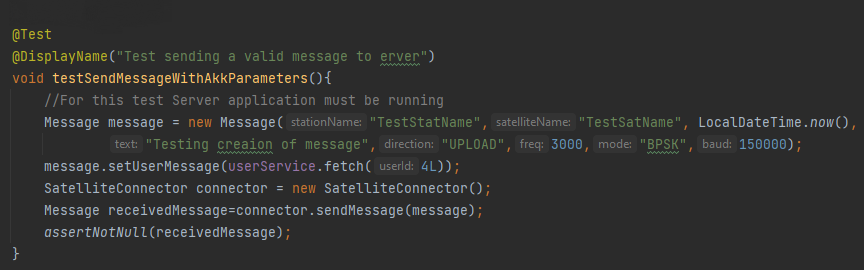
\includegraphics[width=\linewidth]{TestCommunicationWithSatellite2.png}
					\caption{Testiranje ispravne komunikacije sa serverom koji "glumi" satelit.}
					\label{fig:TestCommunicationWithSatellite2}
				\end{figure}
				
			
			
			\subsection{Ispitivanje sustava}
			
            Ispitivanje sustava provedeno je pomoću dodatka za preglednik Selenium IDE. U nastavku su opisani provedeni ispitni slučajevi. \\
            Na slikama \ref{fig:Params1} i \ref{fig:Result1} prikazan je prvi ispitni slučaj u kojem je ispitan pokušaj prijave registriranog korisnika čiji podaci postoje u bazi podataka. Očekivani izlaz je uspješno provedena prijava u sustav i preusmjeravanje na početnu stranicu korisnika. \\

                \begin{figure}[H]
                \centering
				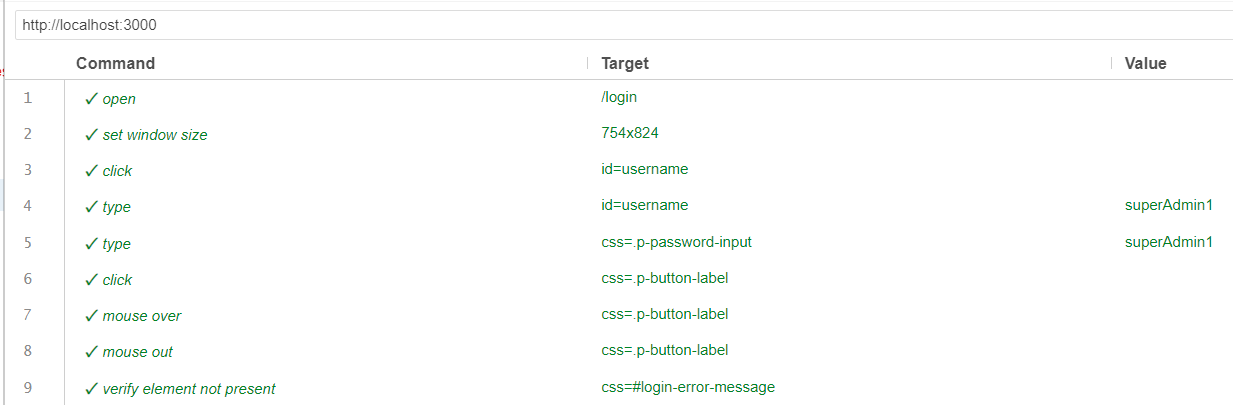
\includegraphics[width=\linewidth]{slike/loginSuccessParams.png}
				\caption{Parametri prvog ispitnog slučaja }
				\label{fig:Params1}
			\end{figure}
   
                 \begin{figure}[H]
                 \centering
				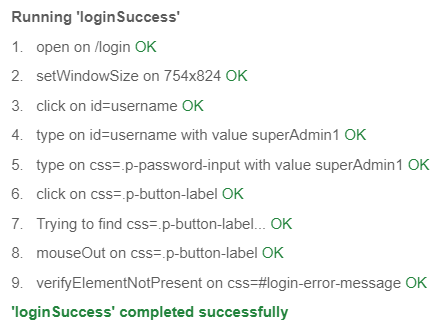
\includegraphics[width=0.5\linewidth]{slike/loginSuccess.png}
				\caption{Rezultat prvog ispitnog slučaja}
				\label{fig:Result1}
			\end{figure}

			\eject
            Slike \ref{fig:Params2} i \ref{fig:Result2} prikazuju drugi ispitni slučaj u kojem je ispitan pokušaj prijave korisnika koji ne postoji u bazi podataka. Očekivani izlaz je neuspješna prijava korisnika u sustav te prikaz poruke pogreške.

                \begin{figure}[H]
                \centering
				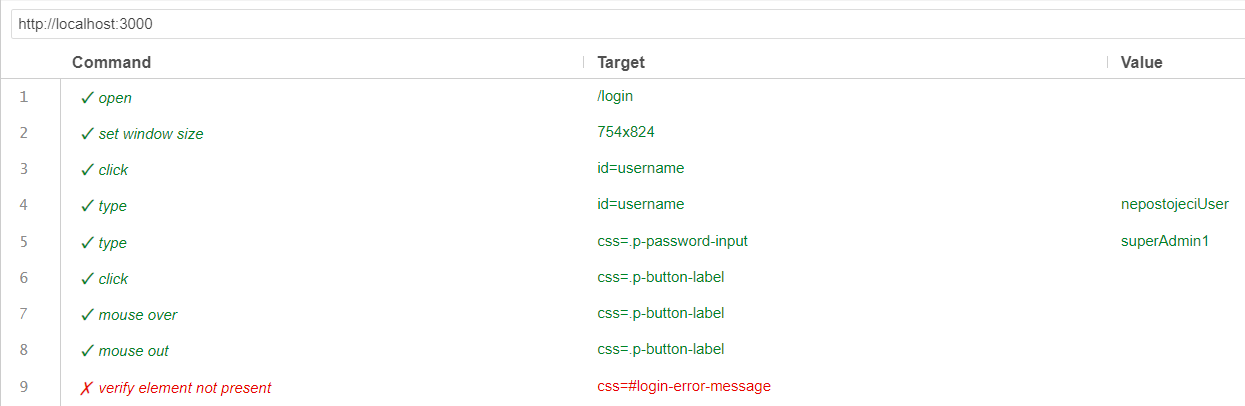
\includegraphics[width=\linewidth]{slike/loginFailParams.png}
				\caption{Parametri drugog ispitnog slučaja }
				\label{fig:Params2}
			\end{figure}
   
                 \begin{figure}[H]
                 \centering
				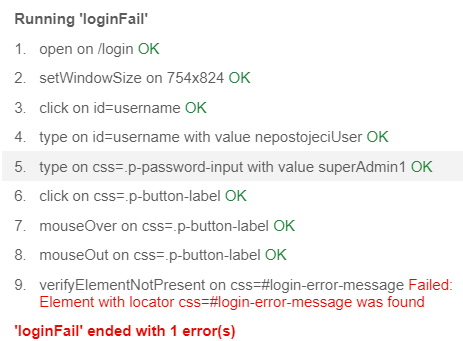
\includegraphics[width=0.5\linewidth]{slike/loginFail.png}
				\caption{Rezultat drugog ispitnog slučaja}
				\label{fig:Result2}
			\end{figure}
			\eject

            Na slikama \ref{fig:Params3} i \ref{fig:Result3} vidimo treći ispitni slučaj koji ispituje registraciju novog korisnika sa valjanim podacima u ispravnom formatu. Očekivani izlaz je uspješna registracija te preusmjeravanje na stranicu Users na kojoj se nalazi lista svih korisnika.

                \begin{figure}[H]
                \centering
				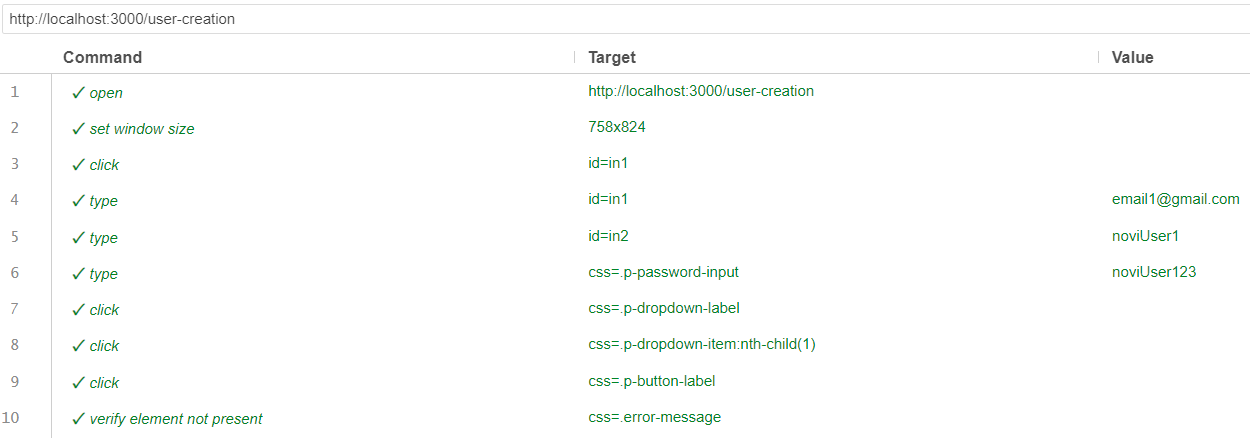
\includegraphics[width=\linewidth]{slike/registerSuccessParams.png}
				\caption{Parametri trećeg ispitnog slučaja }
				\label{fig:Params3}
			\end{figure}
   
                 \begin{figure}[H]
                 \centering
				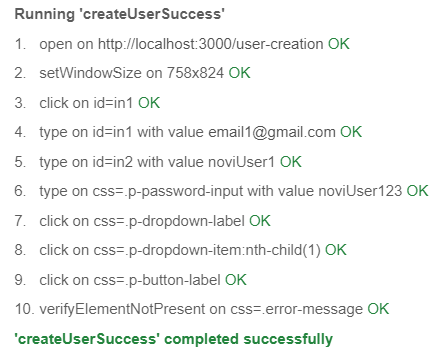
\includegraphics[width=0.5\linewidth]{slike/registerSuccess.png}
				\caption{Rezultat trećeg ispitnog slučaja}
				\label{fig:Result3}
			\end{figure}
			\newpage

            Konačno, Na slikama \ref{fig:Params4} i \ref{fig:Result4} prikazan je četvrti ispitni slučaj u kojem ispitujemo pokušaj registracije korisnika sa neispravnim podacima, odnosno sa e-mail adresom u krivom formatu. Očekivani izlaz je neuspješna registracija te prikaz poruke pogreške.

                \begin{figure}[H]
                \centering
				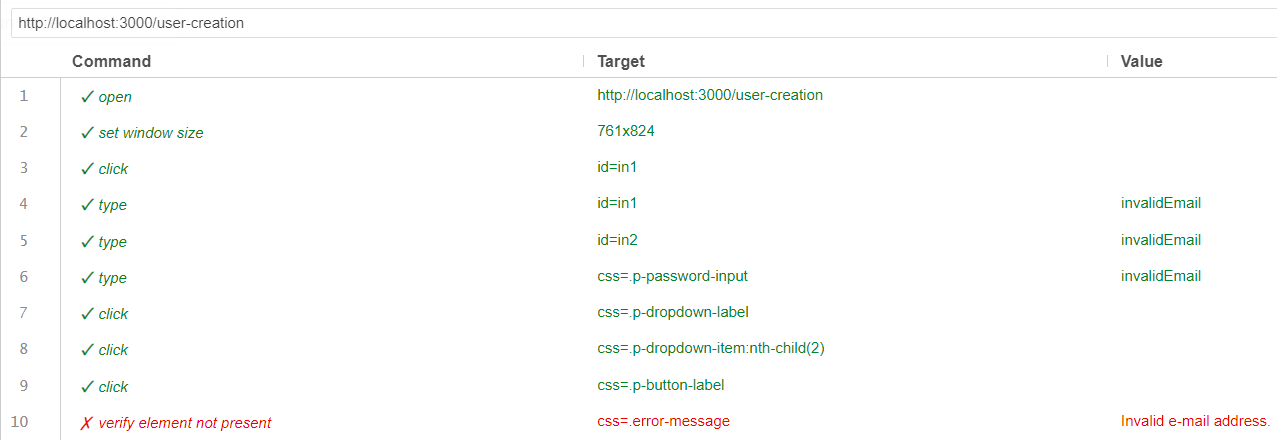
\includegraphics[width=\linewidth]{slike/registerFailParams.png}
				\caption{Parametri četvrtog ispitnog slučaja }
				\label{fig:Params4}
			\end{figure}
   
                 \begin{figure}[H]
                 \centering
				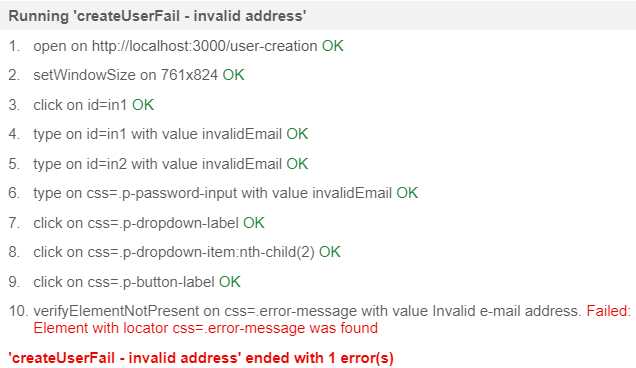
\includegraphics[width=0.5\linewidth]{slike/registerFail.png}
				\caption{Rezultat četvrtog ispitnog slučaja}
				\label{fig:Result4}
			\end{figure}
			
			\eject 
			
		\section{Dijagram razmještaja}
			
			
			
			 Na slici \ref{fig:Dijagram_razmjestaja} prikazan je dijagram razmještaja. Sustav je baziran na arhitekturi "klijent-poslužitelj". Korisnici pristupaju aplikaciji korištenjem web preglednika. Na platformi MicrosoftAzure se nalaze poslužitelji za frontend, backend, bazu podataka te server koji implementira funkcionalnosti satelita. Komunikacija između korisnika i poslužitelja za frontend, te poslužitelja za frontend i poslužitelja za backend, ostvaruje se korištenjem protokola HTTP. Komunikacija između poslužitelja za beckend i servera koji implementira funkcionalnosti satelita odvija se protokolom TCP.
			
			 \begin{figure}[H]
				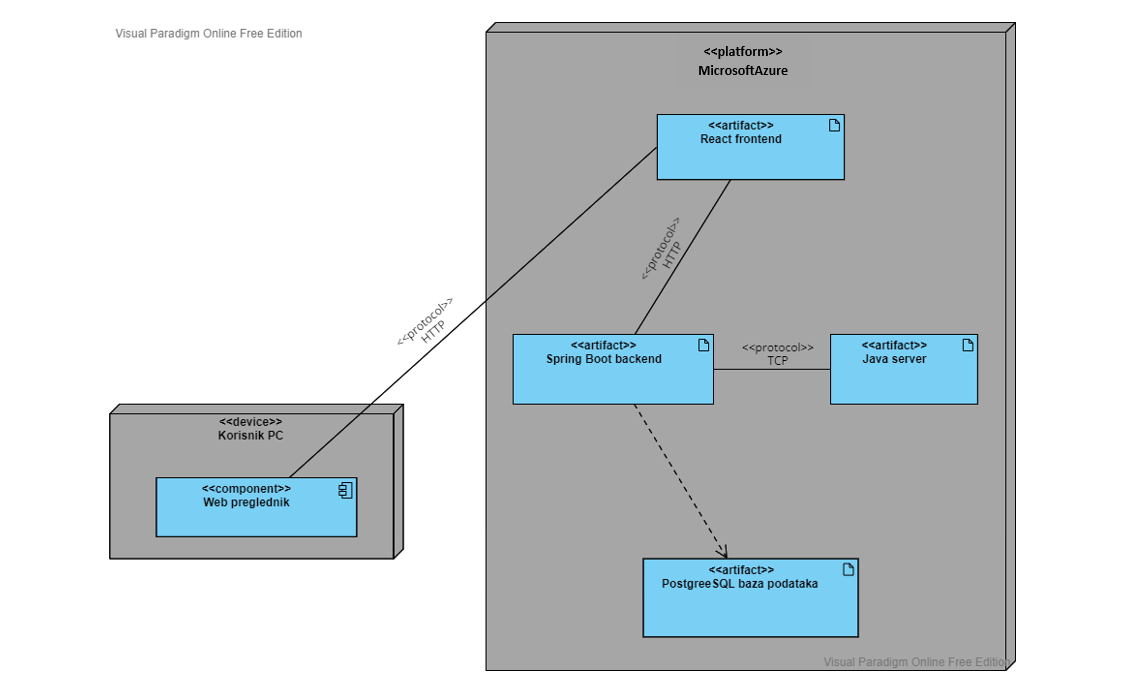
\includegraphics[width=\linewidth]{razmjestaj.png}
				\caption{Dijagram razmještaja}
				\label{fig:Dijagram_razmjestaja}
			\end{figure}
		\newpage
		

			\eject 
		
		\section{Upute za puštanje u pogon}

    Za deploy cjelokupne aplikacije korišten je cloud servis Microsoft Azure čime je omogućeno da aplikacija bude javno dostupna. Na virtualnoj mašini (distribucija Linuxa - Ubuntu 20.04.5), prije samog puštanja aplikacije u pogon, nužno je instalirati potrebnu programsku podršku. Budući da je deployment rađen na virtualnoj mašini u oblaku, sav potrebni softver instaliran je preko komandne linije. U sljedećim odlomcima bit će opisan kompletan postupak postavljanja okruženja za puštanje aplikacije u pogon.
    \newline
    \newline
    \textbf{Konfiguracija backenda}
    
    Za potrebe naše aplikacije nužno je instalirati odgovarajuću Java verziju. U našem slučaju dovoljna je Java 11. Nadalje, potrebno je preuzeti Postgres bazu podataka. Korištena je verzija Postgres 15.1. Uz instalaciju Postgres baze potrebno je provesti standardni setup (stvoriti korisnika, podesiti port, dodijeliti memoriju). Uputstva za setup baze lako je pronaći online u službenoj dokumentaciji.
    
    \begin{figure}[H]
			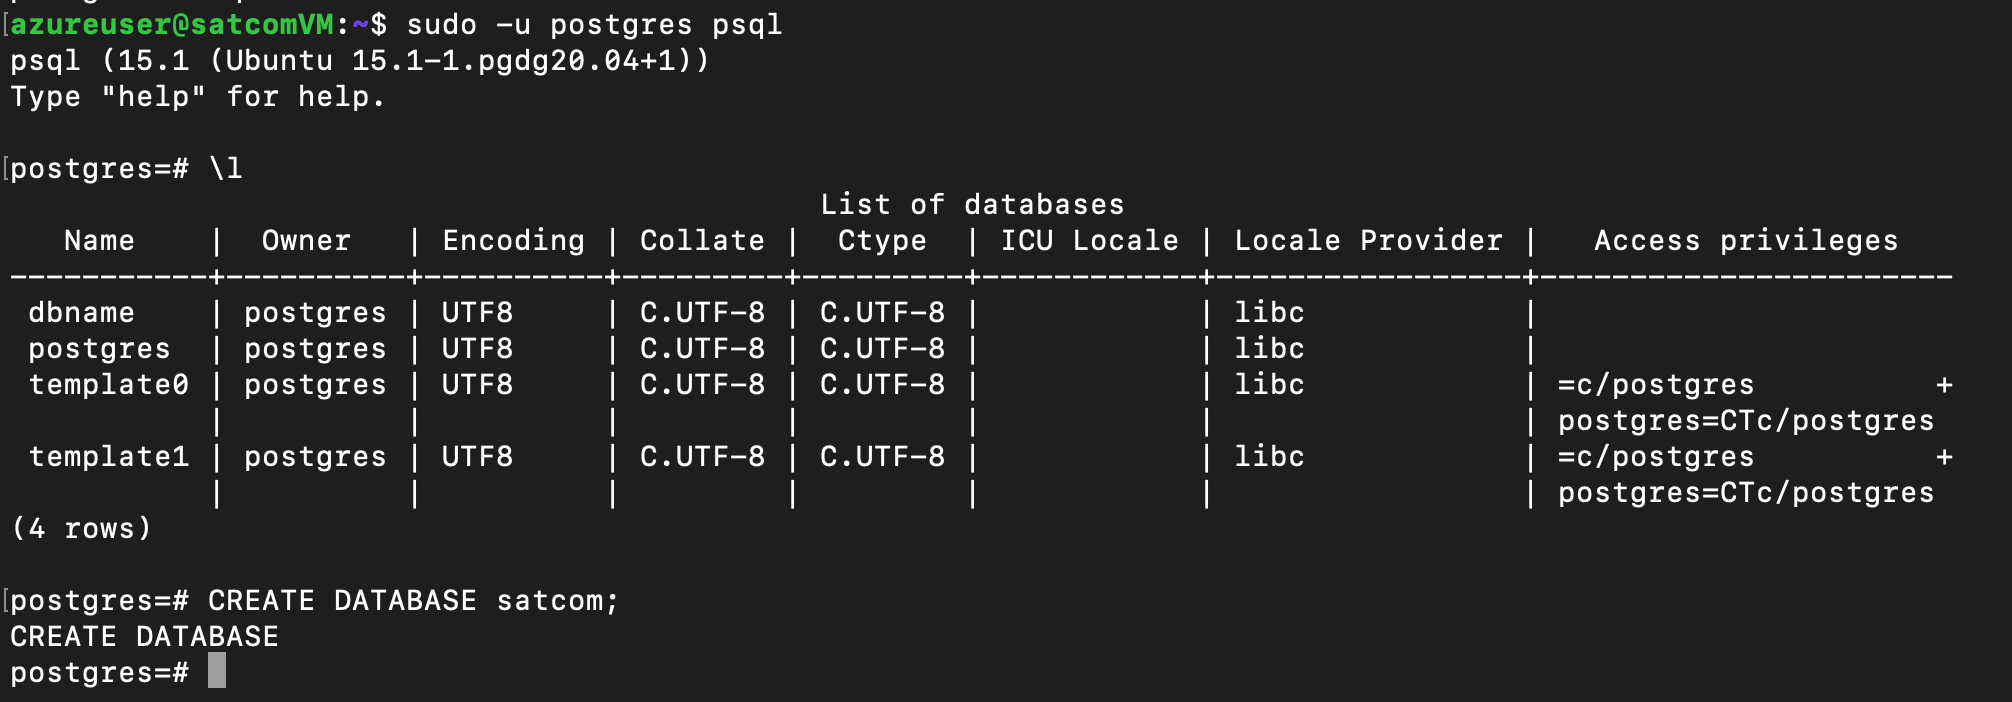
\includegraphics[width=\linewidth]{psql.png}
			\caption{Prikaz konfiguracije baze}
			\label{fig:baza}
		\end{figure}

		Kako bi backend dio aplikacije uspješno spremao i dohvaćao podatke potrebno je u prethodno instaliranoj Postgres bazi prije njegova pokretanja stvoriti bazu podataka pod nazivom 'satcom'. Za to je najjednostavnije koristiti defaultnog postgres korisnika koji dolazi s instalacijom postgres baze podataka te koristeći psql CLI generirati novu bazu podataka preko komandne linije. Ta baza podataka bit će popunjena podacima od strane aplikacije.
    \newline
      \begin{figure}[H]
			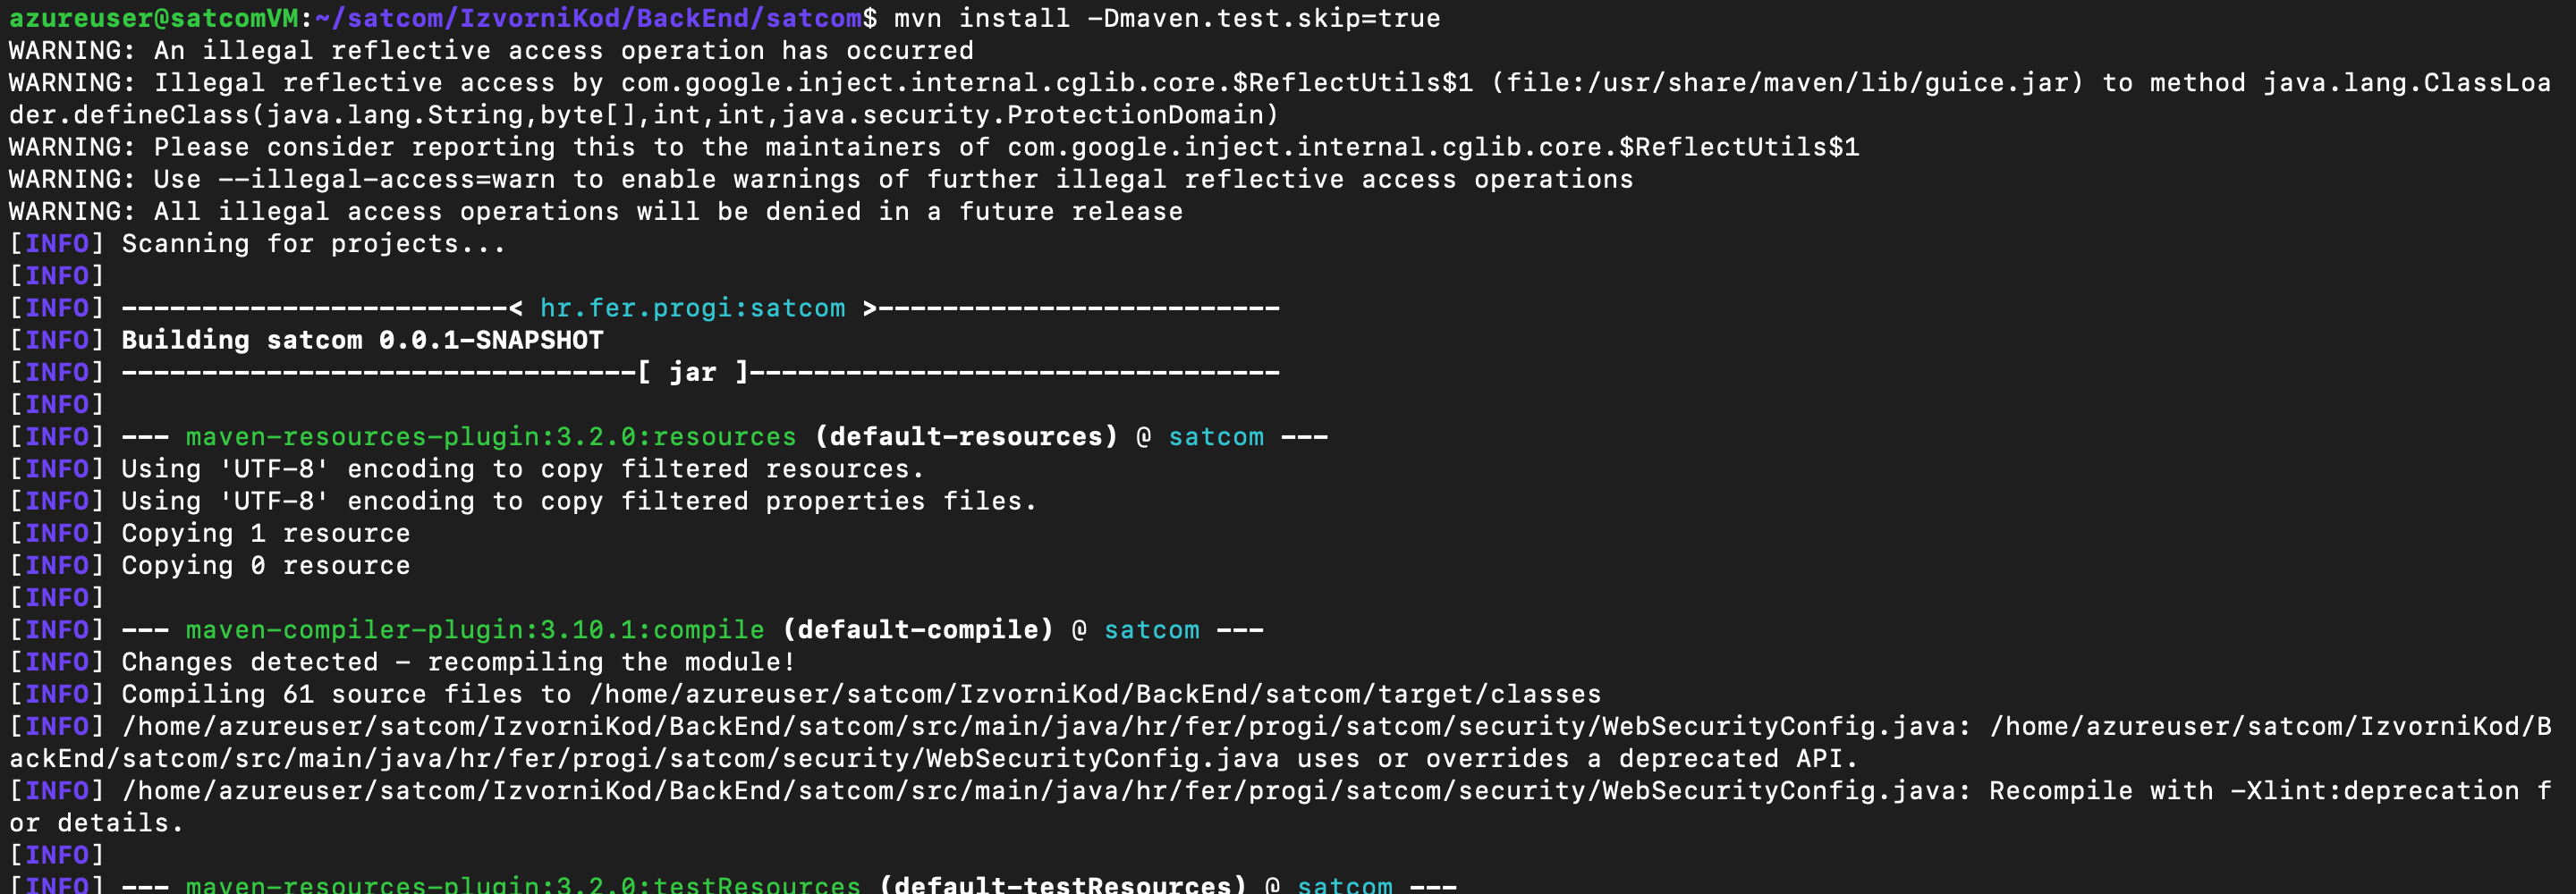
\includegraphics[width=\linewidth]{backend_mvn_install.png}
			\caption{Pokretanje maven builda}
			\label{fig:build}
		\end{figure}

    Za jednostavniji build backenda koristili smo Apache Maven project manager. Njega je također potrebno preuzeti kako bi se cjelokupna aplikacija uspješno izgradila prema postavkama definiranim unutar maven datoteke pom.xml. Ona definira određene ovisnosti (dependencies), build direktorij, izvorni direktorij, testni izvorni direktorij te ostale dodatke (plugins) koji su potrebni našoj aplikaciji da bi funkcionirala.
    \begin{figure}[H]
			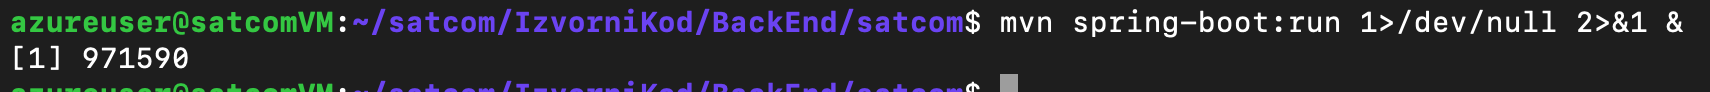
\includegraphics[width=\linewidth]{springboot_run.png}
			\caption{Pokretanje spring aplikacije}
			\label{fig:spring}
		\end{figure}
    

    \textbf{Konfiguracija frontenda}

		Za pokretanje frontend dijela aplikacije također je potrebno instalirati dodatnu programsku podršku. Prvotno je potrebno instalirati Node, također preko komandne linije, a zatim i npm koji služi kao package manager za Node aplikacije.
    \newline
    \newline
    
      \begin{figure}[H]
			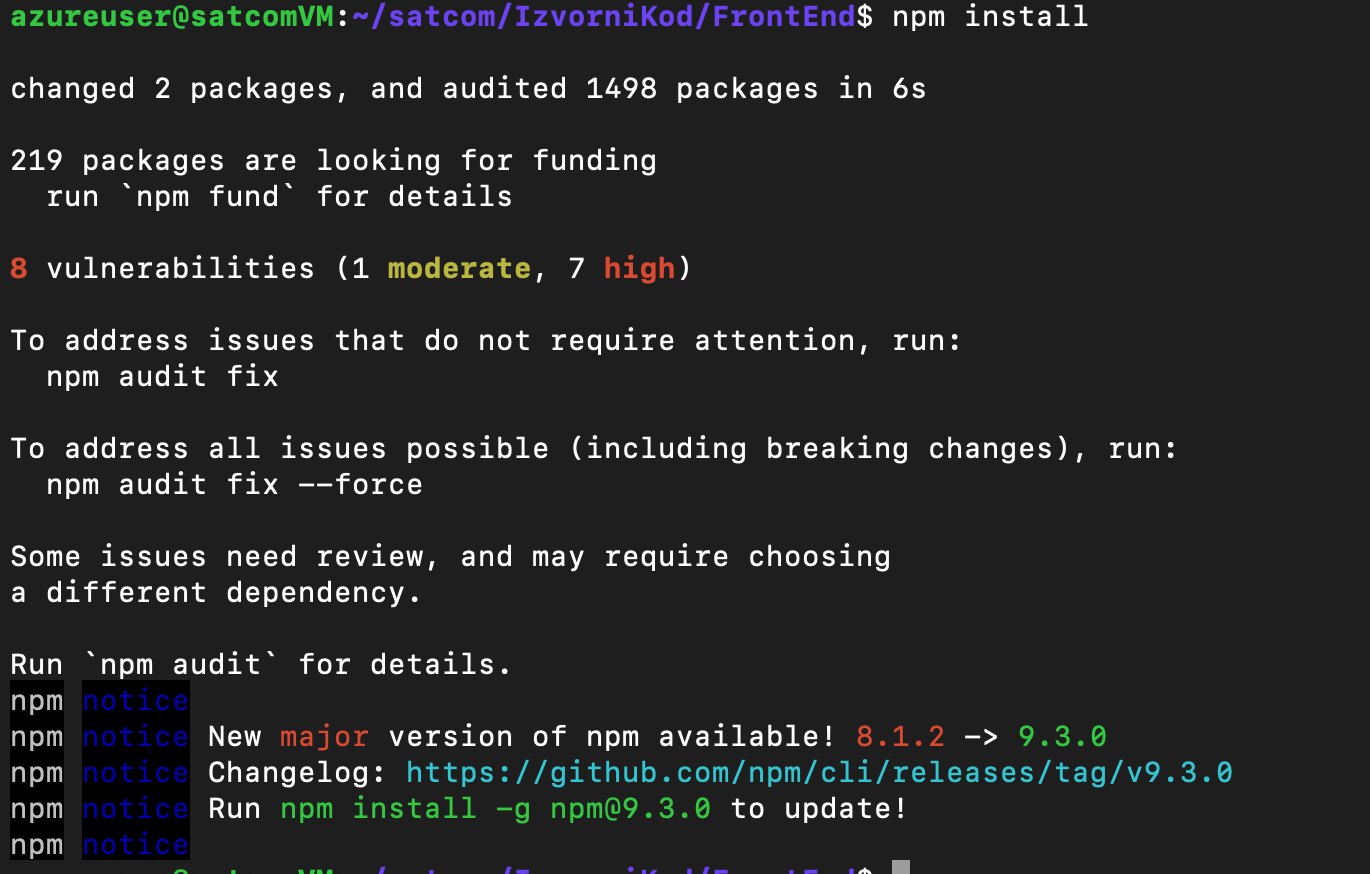
\includegraphics[width=\linewidth]{npm_install.png}
			\caption{Instaliranje node modula}
			\label{fig:npm}
		\end{figure}

    Nakon uspješno provedenih svih navedenih koraka potrebno je povući programski kod s odgovarajućeg git repozitorija.
    \begin{figure}[H]
			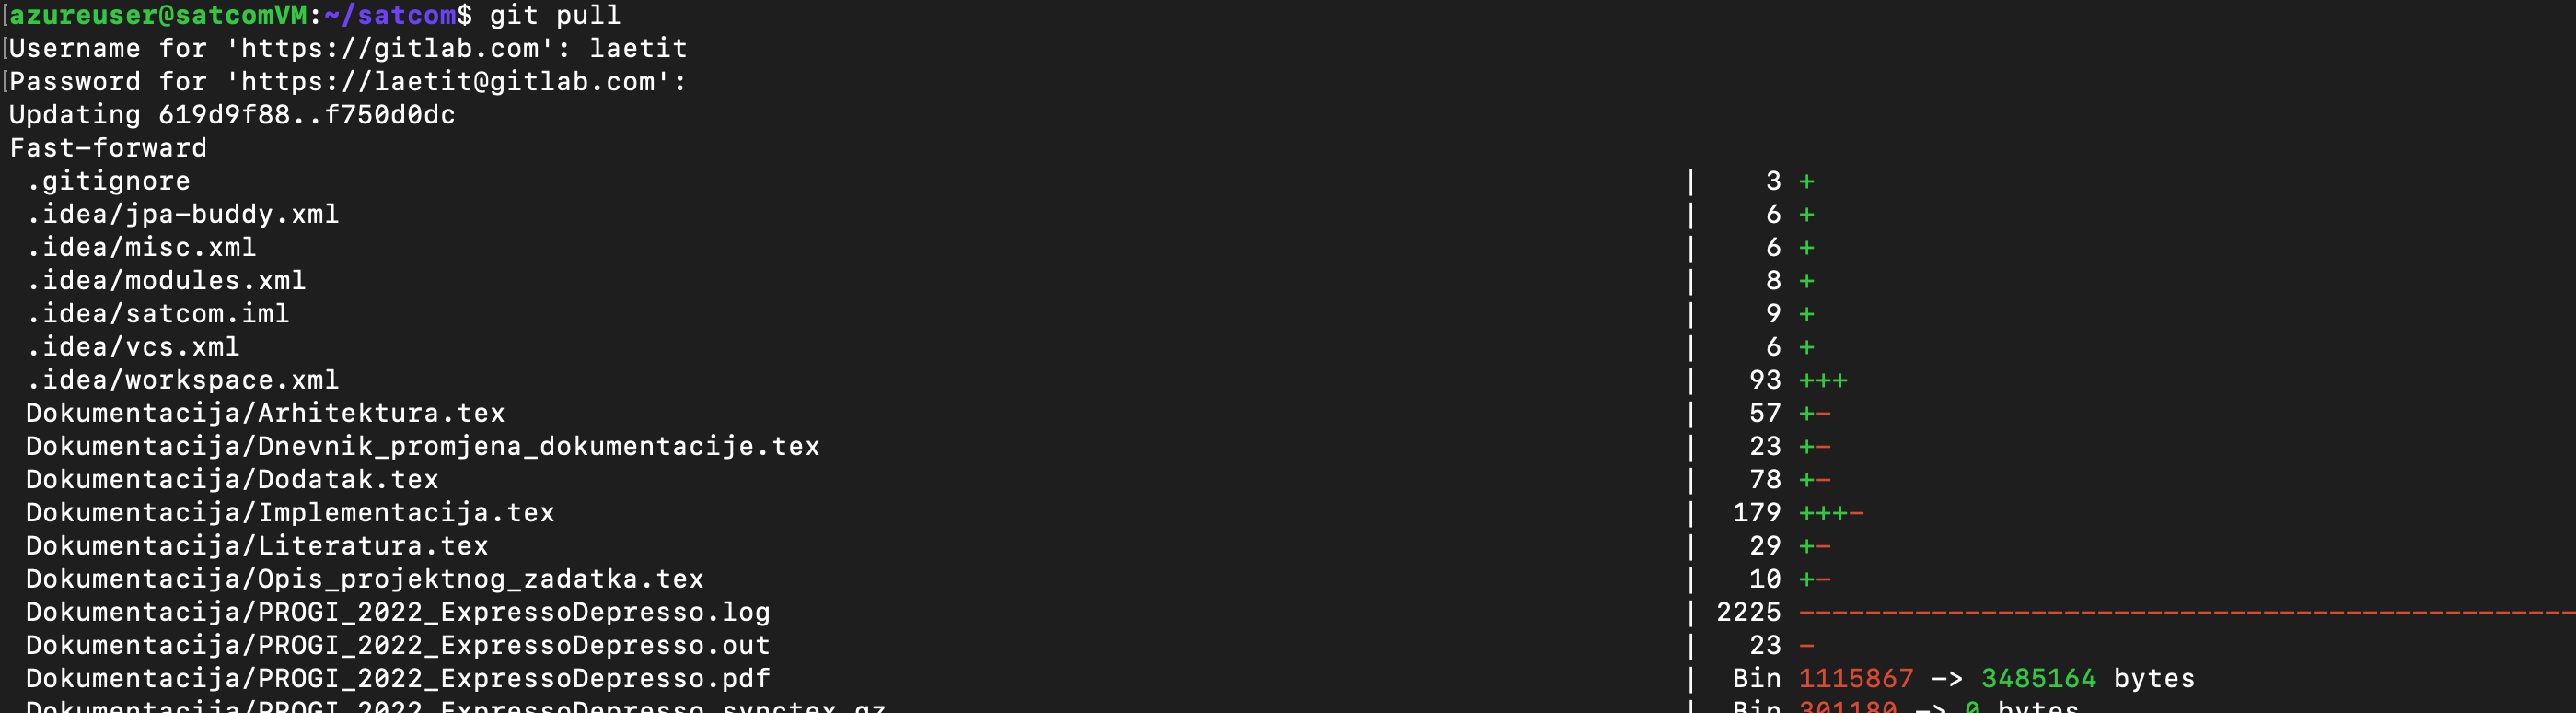
\includegraphics[width=\linewidth]{pull.png}
			\caption{Prikaz pullanja koda s gita}
			\label{fig:pull}
		\end{figure}
  Nakon uspješnog pulla imamo sve potrebne resurse za pokretanje aplikacije te je samo potrebno runnati maven projekte i node aplikaciju u odgovarajućim direktorijima na virtualnoj mašini. Poželjno je aplikaciju staviti da se vrti kao pozadinski proces na virtualnoj mašini.

			\eject 